
\begin{figure}[!ht]
	\centering
	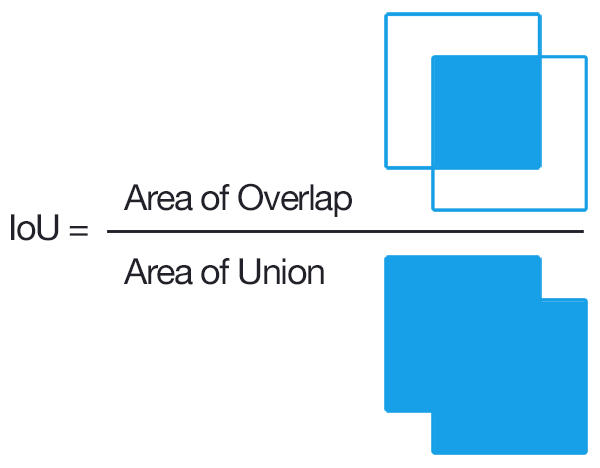
\includegraphics[scale=0.5]{chapter2/images/iou_equation.png}
		\caption{ตัวอย่างการเคลื่อนที่ของลูกบอล}
    	\label{fig:iou_equation}
\end{figure}

เป็นหนึ่งวิธีในการประเมินผลการทดลองสำหรับการตรวจจับวัตถุ โดยหลักการของการคำนวณ IoU สำหรับการประเมินผลการตรวจจับวัตถุ คือ การนำกรอบสี่เหลี่ยมจริงของเฟรม และ กรอบสี่เหลี่ยมที่ทำนายขึ้นมา มาหาอัตราส่วนระหว่าง พื้นที่ที่กรอบสี่เหลี่ยมทั้งสองทับซ้อนกัน และ พื้นที่ทั้งหมดของกรอบสี่เหลี่ยมทั้งสองรวมกัน ผลลัพธ์จะได้เป็นค่า IoU ซึ่งจะมีสมการดังนี้
\begin{equation}
IoU(P,G) = \frac{\left| P \cap G \right|}{\left| P \cup  G \right|}					
\end{equation}
โดยที่
\begin{conditions}
IoU			&  ค่าที่ใช้สำหรับวัดผลความใกล้เคียงระหว่างสองกรอบสี่เหลี่ยม    \\
P			&  พื้นที่ของกรอบสี่เหลี่ยมที่ทำนายได้	\\
G			&  พื้นที่ของกรอบสี่เหลี่ยมจริงของรูปภาพ					\\
\end{conditions}
